\section{View from above}

\subsection{Domain of use}
\begin{frame}
	\frametitle{Application domain and working principle}
	
	\begin{itemize}
		\item Industrial environment.\\
		\item An energy meter sends data regarding the electric consumption of a machinery through the internet.\\
		\item Data are received, analysed and collected by the cloud application.
	\end{itemize}
	
	\bigskip
	\begin{figure}[h]
		\centering
		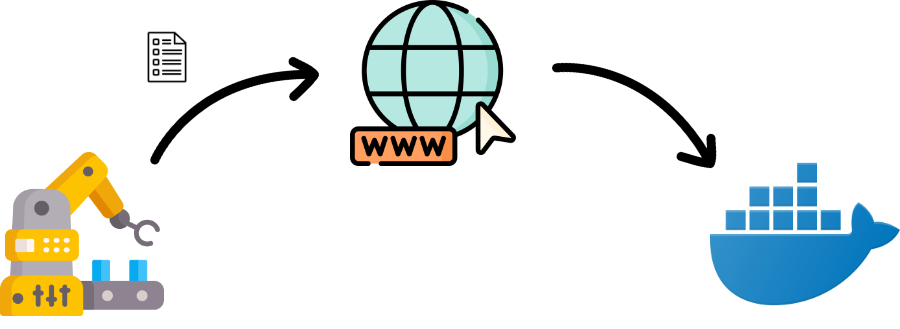
\includegraphics[width=0.5\textwidth]{./img/general_domain.png}
	\end{figure}
\end{frame}


\subsection{General structure}
\begin{frame}
	\frametitle{General structure of the system}
	
	\begin{itemize}
		\item 5 microservices.
		\item Every microservice carry on a specific task.
		\item Only one entry point.
	\end{itemize}
	
	\begin{figure}[h]
		\centering
		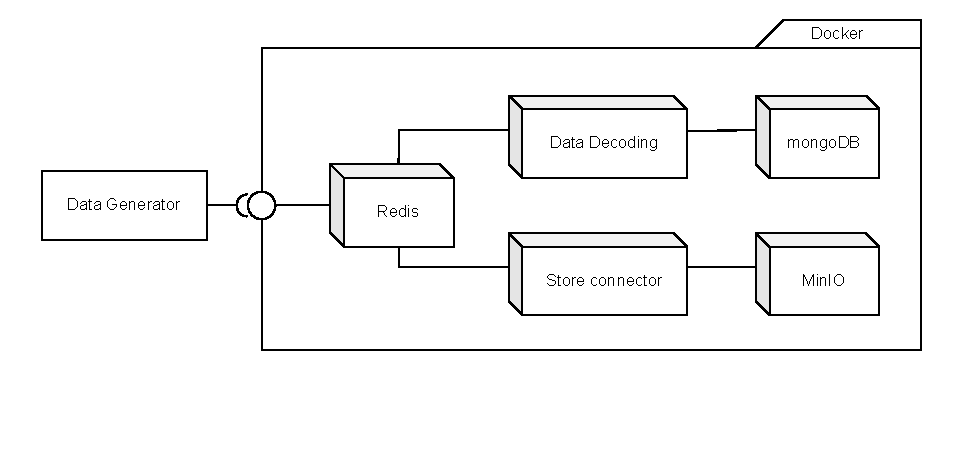
\includegraphics[width=0.8\textwidth]{./drawings/general_scheme.pdf}
	\end{figure}
\end{frame}


\subsection{Docker}
\begin{frame}
    \frametitle{Docker}
    
    \begin{itemize}
        \item It is a set of \emph{platform as a service} (PaaS) products.
        \item It uses OS-level virtualization to execute software inside packages called \emph{containers}.
        \item A container encapsulates its own software, libraries and configuration files.
        \item A container can communicate with other services through well defined channels.
        \item Each container execute the application in an isolated environment.
    \end{itemize}
    
    \begin{figure}[h]
        \centering
        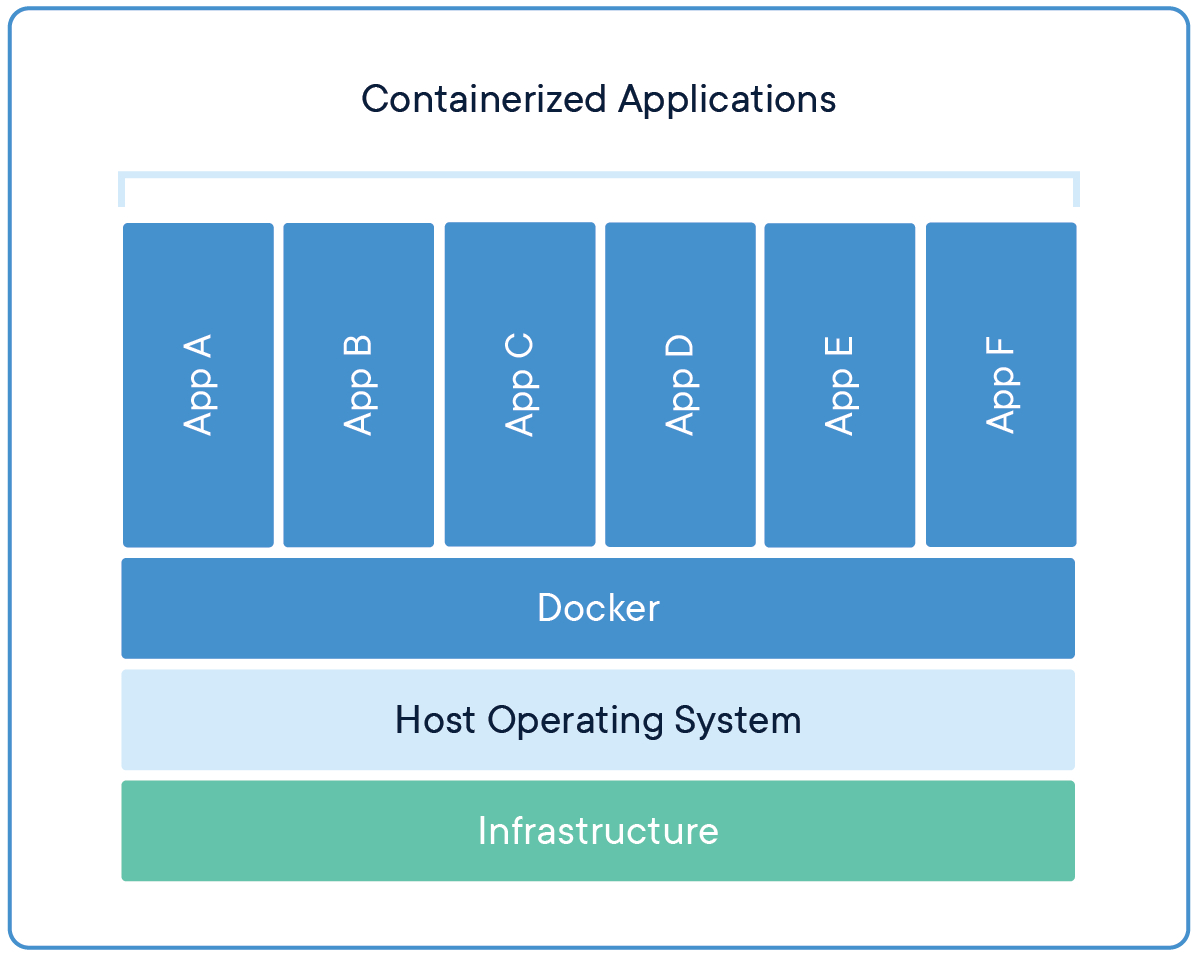
\includegraphics[width=0.3\textwidth]{./img/docker-containers.jpg}
    \end{figure}
\end{frame}

